\documentclass{article}
\usepackage{amsmath}
\usepackage{amssymb}
\usepackage{hyperref}
\usepackage{pdfpages}

\title{Assignment 2A}
\author{Botond Lovász}
\date{\today}

\begin{document}

\maketitle

\section*{Question 2.1.1: Bernoulli Distribution}

\textbf{Given:}
\begin{itemize}
    \item \( \theta = p \)
    \item \( \eta(\theta) = \log \frac{\theta}{1-\theta} \)
    \item \( h(x) = 1 \)
    \item \( T(x) = x \)
    \item \( A(\eta) = \log(1 + e^\eta) \)
\end{itemize}

\textbf{Derivation:}

Exponential family form:
\[
p(x|\theta) = h(x) \exp(\eta(\theta) \cdot T(x) - A(\eta))
\]

Substituting the given functions:
\[
p(x|p) = 1 \cdot \exp\left(x \log \frac{p}{1-p} - \log(1 + e^{\log \frac{p}{1-p}})\right)
\]

Simplifying the expression:
\[
= \exp\left(x \log \frac{p}{1-p} - \log\left(\frac{1}{1-p}\right)\right)
\]
\[
= \exp\left(x \log p + (1-x) \log(1-p)\right)
\]
\[
= p^x (1-p)^{1-x}
\]

This matches the PMF of the Bernoulli distribution.

\section*{Question 2.1.2: Gamma Distribution}

\textbf{Given:}
\begin{itemize}
    \item \( \theta = [\alpha, \beta] \)
    \item \( \eta(\theta) = [\theta_1 - 1, -\theta_2] \)
    \item \( h(x) = 1 \)
    \item \( T(x) = [\log x, x] \)
    \item \( A(\eta) = \log \Gamma(\eta_1 + 1) - (\eta_1 + 1) \log(-\eta_2) \)
\end{itemize}

\textbf{Derivation:}

Exponential family form:
\[
p(x|\theta) = h(x) \exp(\eta(\theta) \cdot T(x) - A(\eta))
\]

Substituting the given functions:
\[
p(x|\alpha, \beta) = 1 \cdot \exp\left((\alpha-1) \log x - \beta x - \log \Gamma(\alpha) + \alpha \log \beta\right)
\]
\[
= \frac{\beta^\alpha}{\Gamma(\alpha)} x^{\alpha-1} e^{-\beta x}
\]

This matches the PDF of the Gamma distribution.

\section*{Question 2.1.3: Log-Normal Distribution}

\textbf{Given:}
\begin{itemize}
    \item \( \theta = [\mu, \sigma^2] \)
    \item \( \eta(\theta) = \left[ \frac{\theta_1}{\theta_2}, -\frac{1}{2\theta_2} \right] \)
    \item \( h(x) = \frac{1}{x\sqrt{2\pi}} \)
    \item \( T(x) = [\log x, (\log x)^2] \)
    \item \( A(\eta) = -\frac{\eta_1^2}{4\eta_2} - \frac{1}{2} \log(-2\eta_2) \)
\end{itemize}

\textbf{Derivation:}

Exponential family form:
\[
p(x|\theta) = h(x) \exp(\eta(\theta) \cdot T(x) - A(\eta))
\]

Substituting the given functions:
\[
p(x|\mu, \sigma^2) = \frac{1}{x\sqrt{2\pi}} \exp\left(\frac{2\mu}{2\sigma^2} \log x - \frac{1}{2\sigma^2} (\log x)^2 - \frac{\mu^2}{2\sigma^2} + \frac{1}{2} \log(\frac{1}{\sigma^2})\right)
\]
\[
= \frac{1}{x\sigma\sqrt{2\pi}} \exp\left(-\frac{(\log x - \mu)^2}{2\sigma^2}\right)
\]

This matches the PDF of the Log-Normal distribution.

\section*{Question 2.1.4: Beta Distribution}

\textbf{Given:}
\begin{itemize}
    \item \( \theta = [\psi_1, \psi_2] \)
    \item \( \eta(\theta) = [\theta_1 - 1, \theta_2 - 1] \)
    \item \( h(x) = 1 \)
    \item \( T(x) = [\log x, \log(1 - x)] \)
    \item \( A(\eta) = \log \Gamma(\eta_1 + 1) + \log \Gamma(\eta_2 + 1) - \log \Gamma(\eta_1 + \eta_2 + 2) \)
\end{itemize}

\textbf{Derivation:}

Exponential family form:
\[
p(x|\theta) = h(x) \exp(\eta(\theta) \cdot T(x) - A(\eta))
\]

Substituting the given functions:
\[
p(x|\psi_1, \psi_2) = 1 \cdot \exp\left((\psi_1-1) \log x + (\psi_2-1) \log(1-x) - \log \Gamma(\psi_1) - \log \Gamma(\psi_2) + \log \Gamma(\psi_1 + \psi_2)\right)
\]
\[
= \frac{\Gamma(\psi_1 + \psi_2)}{\Gamma(\psi_1)\Gamma(\psi_2)} x^{\psi_1-1} (1-x)^{\psi_2-1}
\]

This matches the PDF of the Beta distribution.

\section*{Question 2.2.5: Definition of Local Hidden Variables}

\[
p(x_n, z_n | x_{-n}, z_{-n}, \beta, \alpha) = p(x_n, z_n | \beta, \alpha)
\]
This indicates that each observation \( x_n \) and its corresponding local hidden variable \( z_n \) are conditionally independent of all other observations and local hidden variables, given the global variables \( \beta \) and fixed parameters \( \alpha \).

\section*{Question 2.2.6: LDA Model and Local Hidden Variables}

In the LDA model, the local hidden variables for a document \(d\) are the topic proportions \(\theta_d\) and the topic assignments \(z_d\). These variables are specific to each document given the global variables.

\[
p(w_d, \theta_d, z_d | w_{-d}, \theta_{-d}, z_{-d}, \alpha, \beta) = p(w_d, \theta_d, z_d | \alpha, \beta)
\]

This equality expresses that \(w_{-d}, \theta_{-d}, z_{-d}\) contributes nothing to the certainty of \(w_d, \theta_d, z_d\). In this case, \(w_d, \theta_d, z_d\) and \(w_{-d}, \theta_{-d}, z_{-d}\) are said to be conditionally independent given \(\alpha, \beta\). Which is true given by the nature of the LDA model and data.

\section*{Question 2.2.7: ELBO for the LDA Model}

Source: \url{http://www.cs.columbia.edu/~blei/papers/BleiLafferty2009.pdf}

\[
\mathcal{L} = \sum_{k=1}^{K} \mathbb{E}[\log p(\beta_k | \eta)] + \sum_{d=1}^{D} \mathbb{E}[\log p(\theta_d | \alpha)] + \sum_{d=1}^{D} \sum_{n=1}^{N} \mathbb{E}[\log p(z_{d,n} | \theta_d)]
\]
\[
+ \sum_{d=1}^{D} \sum_{n=1}^{N} \mathbb{E}[\log p(w_{d,n} | z_{d,n}, \beta_{1:K})] + H(q)
\]

\textbf{Final ELBO Expression (taken from the code):}

\[
\mathcal{L} = \sum_{d=1}^{D} \sum_{n=1}^{N} \sum_{k=1}^{K} \phi_{d,n,k} \left( \sum_{w=1}^{W} w_{d,n,w} \left( \Psi(\lambda_{k,w}) - \Psi\left(\sum_{y=1}^{W} \lambda_{k,y}\right) \right) + \Psi(\gamma_{d,k}) - \Psi\left(\sum_{j=1}^{K} \gamma_{d,j}\right) - \log \phi_{d,n,k} \right) \\
\]
\[
- D \cdot \log B(\alpha) + \sum_{d=1}^{D} \sum_{k=1}^{K} (\alpha - 1) \left( \Psi(\gamma_{d,k}) - \Psi\left(\sum_{j=1}^{K} \gamma_{d,j}\right) \right) \\
\]
\[
- K \cdot \log B(\eta) + \sum_{k=1}^{K} \sum_{w=1}^{W} (\eta - 1) \left( \Psi(\lambda_{k,w}) - \Psi\left(\sum_{y=1}^{W} \lambda_{k,y}\right) \right) \\
\]
\[
+ \sum_{d=1}^{D} \left( \log B(\gamma_d) + \left(\sum_{k=1}^{K} \gamma_{d,k} - K\right) \Psi\left(\sum_{k=1}^{K} \gamma_{d,k}\right) - \sum_{k=1}^{K} (\gamma_{d,k} - 1) \Psi(\gamma_{d,k}) \right) \\
\]
\[
+ \sum_{k=1}^{K} \left( \log B(\lambda_k) + \left(\sum_{w=1}^{W} \lambda_{k,w} - W\right) \Psi\left(\sum_{w=1}^{W} \lambda_{k,w}\right) - \sum_{w=1}^{W} (\lambda_{k,w} - 1) \Psi(\lambda_{k,w}) \right)
\]

\section*{Question 2.3.10: Rao-Blackwellization in BBVI}

"Rao-Blackwellization" means transforming an estimator to reduce its variance.
In the BBVI paper, we want to focus on each component of the gradient separately. They reduce the variance by analytically integrating out some of the latent variables which then not need to be sampled, thus reducing it's variance.
Source: \url{https://www.youtube.com/watch?v=GMqwngEdkao&list=PLJ71tqAZr196GJ5G36s64xifr1tURUCSJ&index=9}

\appendix
\section{Jupyter Notebook}
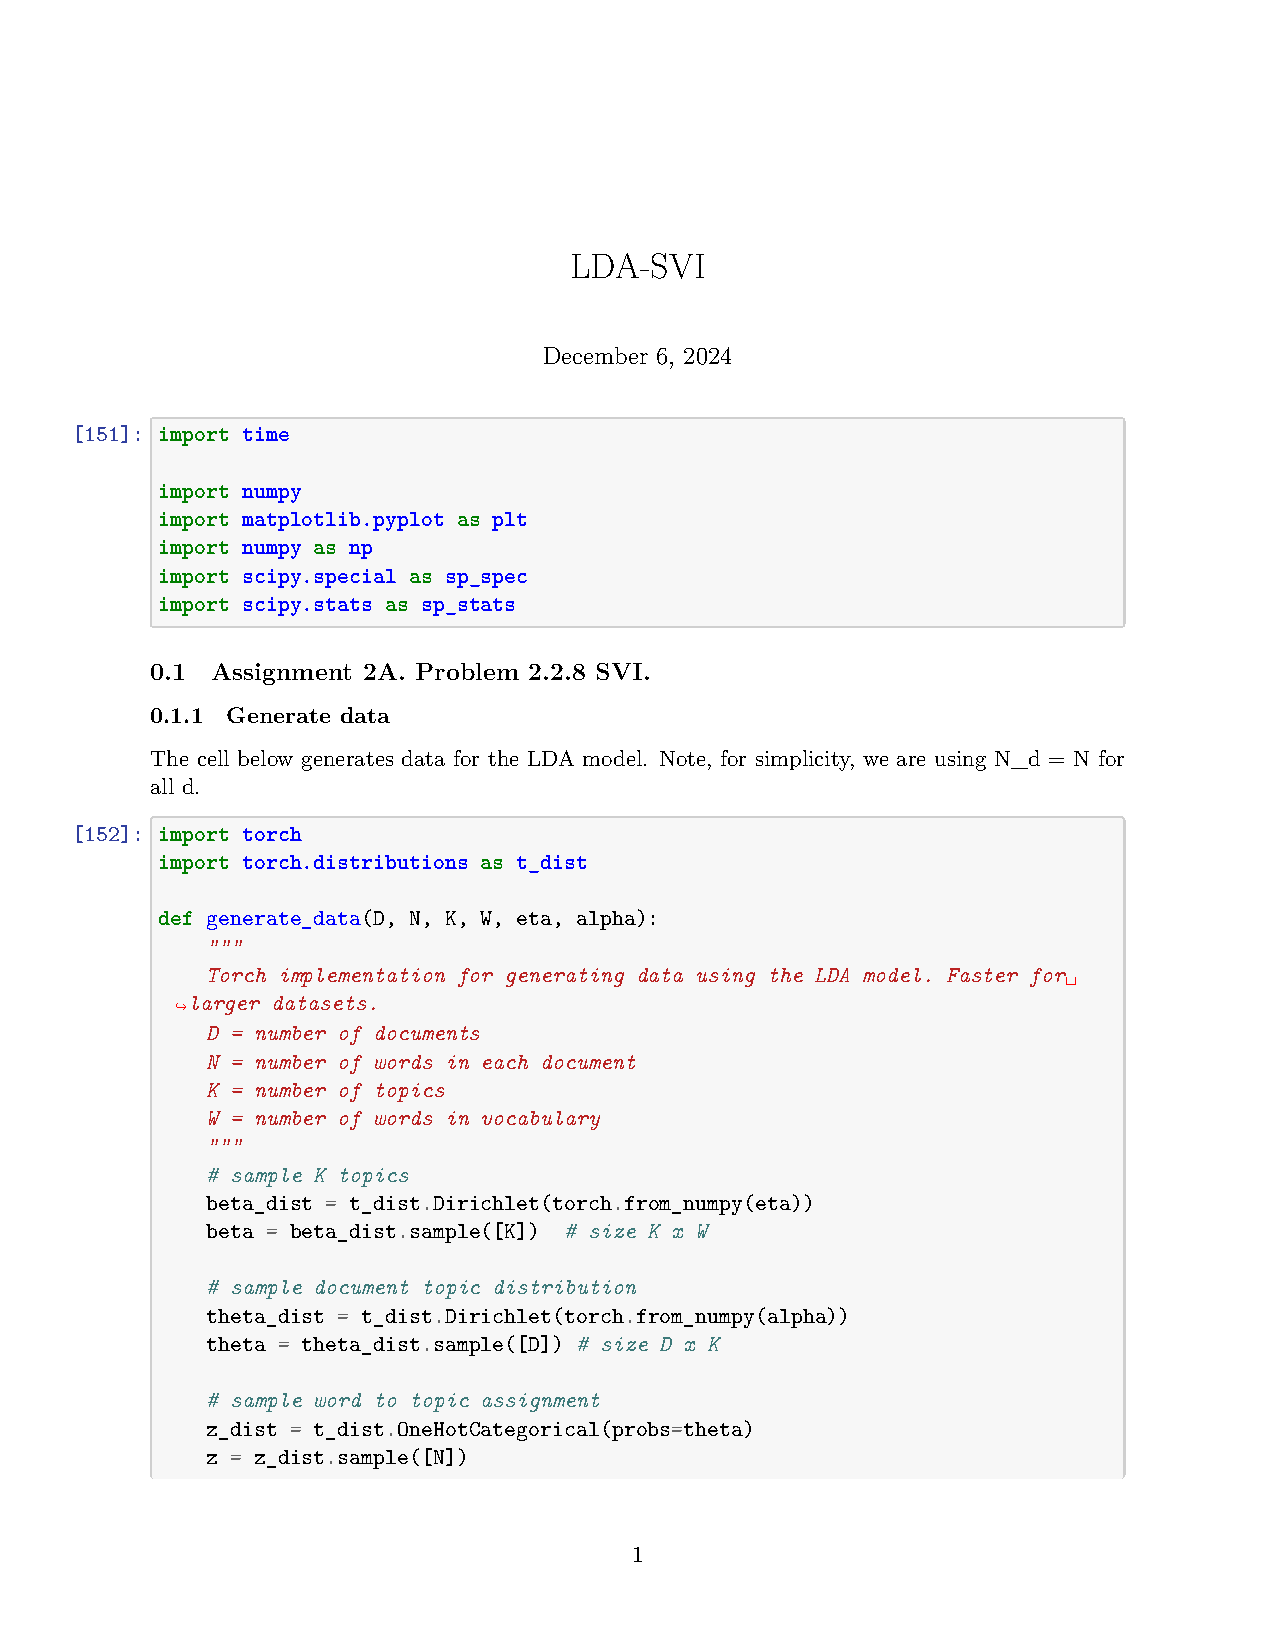
\includepdf[pages=-, scale=0.8]{LDA-SVI.pdf}

\end{document}